% Propósito: clasificar una onda comparando la dirección del movimiento local
% con la dirección de propagación.
% Origen: definiciones de la sección \ref{sec:u3-longitudinal-transversal}.
% Esquema conceptual, no representa datos medidos ni está dibujado a escala.
% Descripción accesible: en el panel superior, las partículas de una onda
% longitudinal se desplazan horizontalmente, en paralelo a la propagación. En
% el panel inferior, una cuerda se desplaza verticalmente mientras la onda se
% propaga horizontalmente.
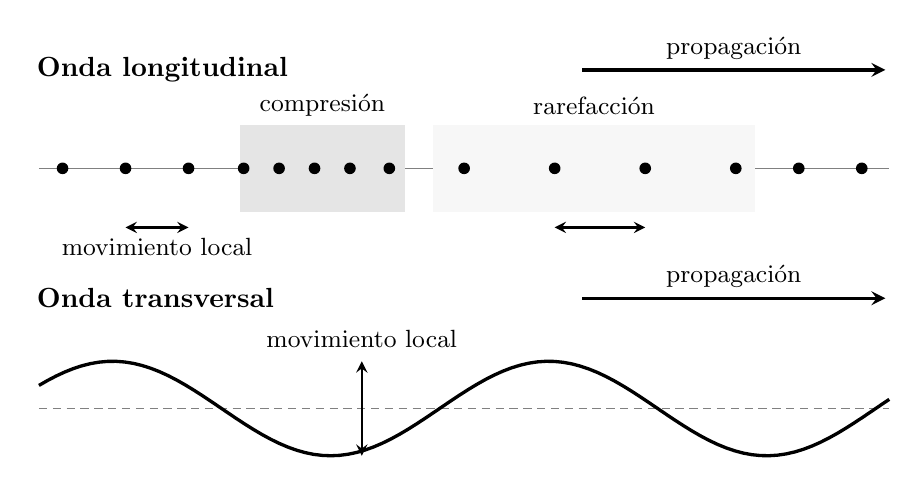
\begin{tikzpicture}[font=\small,>=stealth,x=1cm,y=1cm]
    \node[anchor=west,font=\bfseries] at (0.3,2.10)
        {Onda longitudinal};
    \draw[->,very thick] (7.35,2.10) -- (11.20,2.10)
        node[midway,above] {propagación};

    \draw[gray] (0.45,0.85) -- (11.25,0.85);
    \fill[black!10] (3.00,0.30) rectangle (5.10,1.40);
    \fill[black!3] (5.45,0.30) rectangle (9.55,1.40);
    \node at (4.05,1.65) {compresión};
    \node at (7.50,1.65) {rarefacción};
    \foreach \x in {0.75,1.55,2.35,3.05,3.50,3.95,4.40,4.90,5.85,7.00,8.15,9.30,10.10,10.90}{
        \fill (\x,0.85) circle (2.1pt);
    }
    \draw[<->,thick] (1.55,0.10) -- (2.35,0.10)
        node[midway,below] {movimiento local};
    \draw[<->,thick] (7.00,0.10) -- (8.15,0.10);

    \node[anchor=west,font=\bfseries] at (0.3,-0.80)
        {Onda transversal};
    \draw[->,very thick] (7.35,-0.80) -- (11.20,-0.80)
        node[midway,above] {propagación};
    \draw[densely dashed,gray] (0.45,-2.20) -- (11.25,-2.20);
    \draw[very thick,samples=100,domain=0.45:11.25]
        plot (\x,{-2.20+0.60*sin(65*\x)});
    \draw[<->,thick] (4.55,-2.80) -- (4.55,-1.60);
    \node[above] at (4.55,-1.55) {movimiento local};
\end{tikzpicture}
